\subsection{\textbf{Распределение Максвелла по модулю скорости.} Наиболее вероятная, средняя и средняя квадратичная скорости}
\begin{figure}
	\centering
	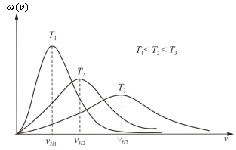
\includegraphics[width=0.5\linewidth]{image/Максвел}
	\caption{Распределение Максвелла по модулю скорости}
	\label{fig:11}
\end{figure}

\subsubsection*{Распределение Максвелла по модулю скорости}
\textbf{Задача: }Найти плотность вероятности $\omega(v)$, которая определяет вероятность того, что скорость молекулы находится в интервале $[v; \, v + dv]$.
\begin{align} \label{17.1}
	\boxed{\omega(v) = 4 \pi v^2 \left(\frac{m}{2\pi k T}\right)^{\frac{3}{2}} \exp \left(-\frac{mv^2}{2kT}\right)}
\end{align}

\[\int_{0}^{\infty} \omega(v) \, dv = 1\]

\textbf{Наиболее вероятный исход }-- это скорость, при которой функция распределения достигает максимума.
\begin{align*}
	v_\text{вер.} = \sqrt{\frac{2RT}{\mu}} && \langle v \rangle = \int_{0}^{\infty} v \cdot \omega(v) \, dv = \sqrt{\frac{8kT}{\pi m}}
\end{align*}

\textbf{Среднеквадратичная скорость:}
\begin{align*}
	v_\text{кв} = \sqrt{\langle v^2 \rangle} && \langle v^2 \rangle = \int_{0}^{\infty} v^2 \omega(v) \, dv = \frac{3kT}{m}
\end{align*}
\[\langle v^2 \rangle = \langle v^2_x \rangle + \langle v^2_y \rangle + \langle v^2_z \rangle = \frac{3kT}{m}\]

\textbf{Среднеквадратичная скорость} определяет среднюю кинетическую энергию:
\begin{align*}
	\langle W_\text{кин} \rangle = \langle \frac{mv^2}{2} \rangle = \frac{m}{2} \langle v^2 \rangle = \frac{mv^2_\text{кв}}{2} = \frac{3}{2}kT && \boxed{\langle W_\text{кин} \rangle = \frac{3}{2}kT}
\end{align*}